% Options for packages loaded elsewhere
\PassOptionsToPackage{unicode}{hyperref}
\PassOptionsToPackage{hyphens}{url}
\PassOptionsToPackage{dvipsnames,svgnames,x11names}{xcolor}
%
\documentclass[
  10pt,
  ignorenonframetext,
  fontset=fandol]{beamer}
\usepackage{pgfpages}
\setbeamertemplate{caption}[numbered]
\setbeamertemplate{caption label separator}{: }
\setbeamercolor{caption name}{fg=normal text.fg}
\beamertemplatenavigationsymbolsempty
% Prevent slide breaks in the middle of a paragraph
\widowpenalties 1 10000
\raggedbottom
\setbeamertemplate{part page}{
  \centering
  \begin{beamercolorbox}[sep=16pt,center]{part title}
    \usebeamerfont{part title}\insertpart\par
  \end{beamercolorbox}
}
\setbeamertemplate{section page}{
  \centering
  \begin{beamercolorbox}[sep=12pt,center]{part title}
    \usebeamerfont{section title}\insertsection\par
  \end{beamercolorbox}
}
\setbeamertemplate{subsection page}{
  \centering
  \begin{beamercolorbox}[sep=8pt,center]{part title}
    \usebeamerfont{subsection title}\insertsubsection\par
  \end{beamercolorbox}
}
\AtBeginPart{
  \frame{\partpage}
}
\AtBeginSection{
  \ifbibliography
  \else
    \frame{\sectionpage}
  \fi
}
\AtBeginSubsection{
  \frame{\subsectionpage}
}
\usepackage{amsmath,amssymb}
\usepackage{lmodern}
\usepackage{iftex}
\ifPDFTeX
  \usepackage[T1]{fontenc}
  \usepackage[utf8]{inputenc}
  \usepackage{textcomp} % provide euro and other symbols
\else % if luatex or xetex
  \usepackage{unicode-math}
  \defaultfontfeatures{Scale=MatchLowercase}
  \defaultfontfeatures[\rmfamily]{Ligatures=TeX,Scale=1}
\fi
\usetheme[]{Singapore}
\usecolortheme{seahorse}
\usefonttheme{structurebold}
% Use upquote if available, for straight quotes in verbatim environments
\IfFileExists{upquote.sty}{\usepackage{upquote}}{}
\IfFileExists{microtype.sty}{% use microtype if available
  \usepackage[]{microtype}
  \UseMicrotypeSet[protrusion]{basicmath} % disable protrusion for tt fonts
}{}
\usepackage{xcolor}
\newif\ifbibliography
\setlength{\emergencystretch}{3em} % prevent overfull lines
\providecommand{\tightlist}{%
  \setlength{\itemsep}{0pt}\setlength{\parskip}{0pt}}
\setcounter{secnumdepth}{-\maxdimen} % remove section numbering
\titlegraphic{
\includegraphics[height=1.5cm]{images/First.jpg}}
\logo{
\includegraphics[width=0.6in,height=0.2in]{images/JNU1.jpg}}
\usepackage[fontset = windows]{}
\usepackage{wrapfig}
\usepackage{tikz}
\usepackage{wallpaper}
\usepackage{xcolor}
\usepackage[default]{sourcesanspro}
\usepackage[scale=.9]{sourcecodepro}
\ifLuaTeX
  \usepackage{selnolig}  % disable illegal ligatures
\fi
\usepackage[]{natbib}
\bibliographystyle{apalike}
\IfFileExists{bookmark.sty}{\usepackage{bookmark}}{\usepackage{hyperref}}
\IfFileExists{xurl.sty}{\usepackage{xurl}}{} % add URL line breaks if available
\urlstyle{same} % disable monospaced font for URLs
\hypersetup{
  pdftitle={Interpretable Machine Learning of PET Imaging for Individualized Predictions of Seizure Outcomes after Temporal Lobe Epilepsy Surgery},
  pdfauthor={Huanhua Wu Prof.~Hao Xu\^{}\{*\} ~},
  pdfkeywords={Epilepsy, PET/CT, Radiomics, Explainable Machine
Learning},
  colorlinks=true,
  linkcolor={ForestGreen},
  filecolor={Maroon},
  citecolor={Blue},
  urlcolor={Blue},
  pdfcreator={LaTeX via pandoc}}

\title{Interpretable Machine Learning of PET Imaging for Individualized
Predictions of Seizure Outcomes after Temporal Lobe Epilepsy Surgery}
\author{Huanhua Wu\\
Prof.~Hao Xu\(^{*}\) ~}
\date{2023-02-06}
\institute{The First Affiliated Hospital of Jinan University ~}

\begin{document}
\frame{\titlepage}

\begin{frame}[allowframebreaks]
  \tableofcontents[hideallsubsections]
\end{frame}
\begin{frame}
\setbeamercolor{titlelike}{bg=black,fg=white}
\newcommand\Background{%
\begin{tikzpicture}[remember picture,overlay]
\node[inner sep = 0pt, outer sep = 0pt,opacity=0.65]
  at (current page.center)
  {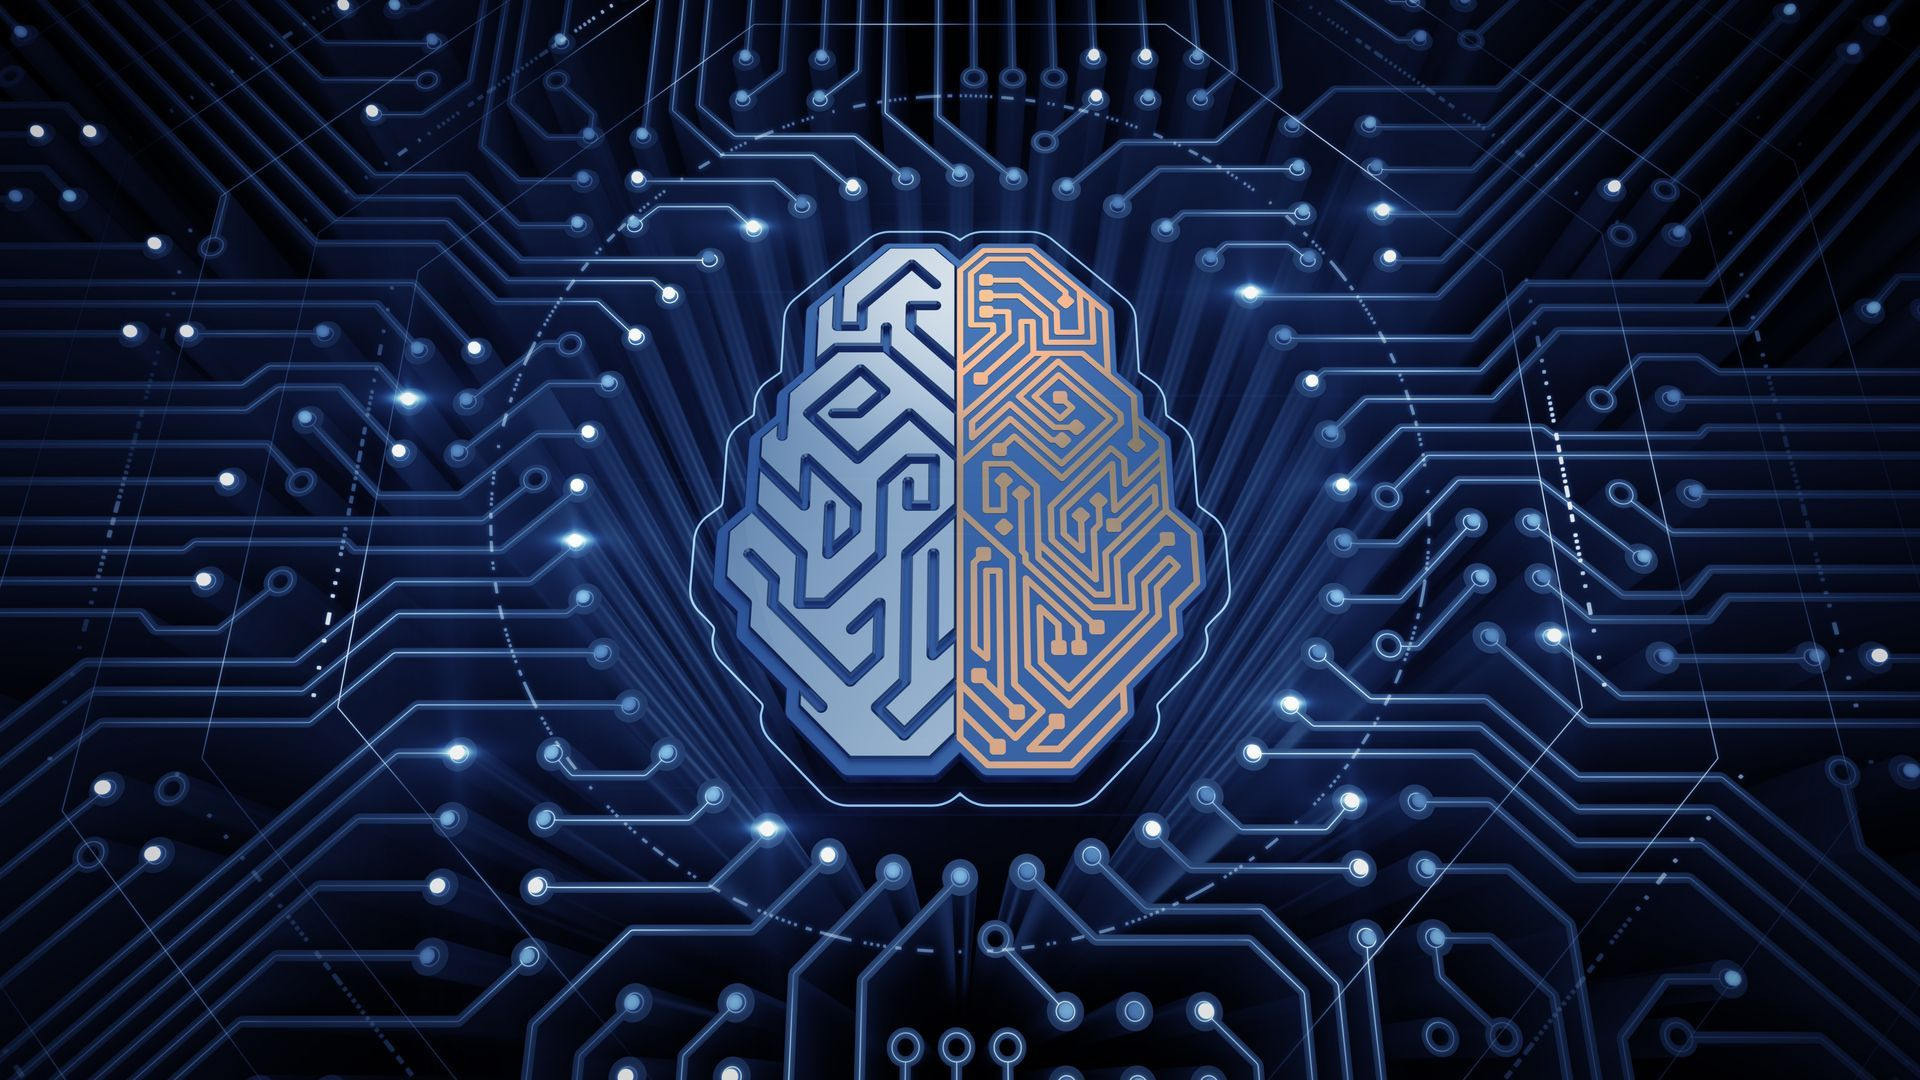
\includegraphics[width=\paperwidth,height=\paperheight]{images/AI.jpg}};
\end{tikzpicture}%
}

\def\begincols{\begin{columns}}
\def\begincol{\begin{column}}
\def\endcol{\end{column}}
\def\endcols{\end{columns}}
\end{frame}

\hypertarget{introduction}{%
\section{Introduction}\label{introduction}}

\begin{frame}{Background}
\protect\hypertarget{background}{}
\begin{figure}

{\centering 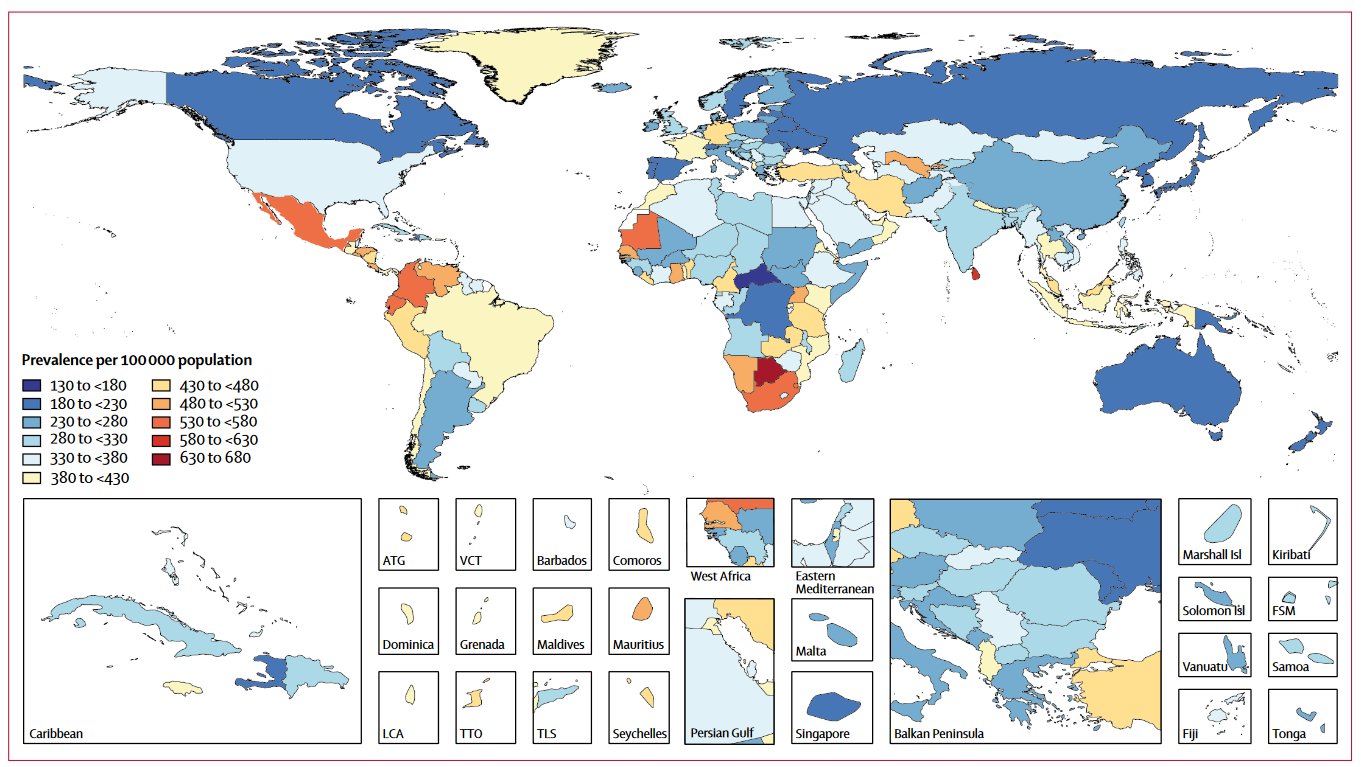
\includegraphics[width=1\linewidth]{images/global_epi} 

}

\caption{Epilepsy Epidemiology}\label{fig:unnamed-chunk-2}
\end{figure}
\end{frame}

\begin{frame}{Aims}
\protect\hypertarget{aims}{}
\begin{columns}
\column{.45\textwidth}
\begin{figure}
\centering
% Requires \usepackage{graphicx}
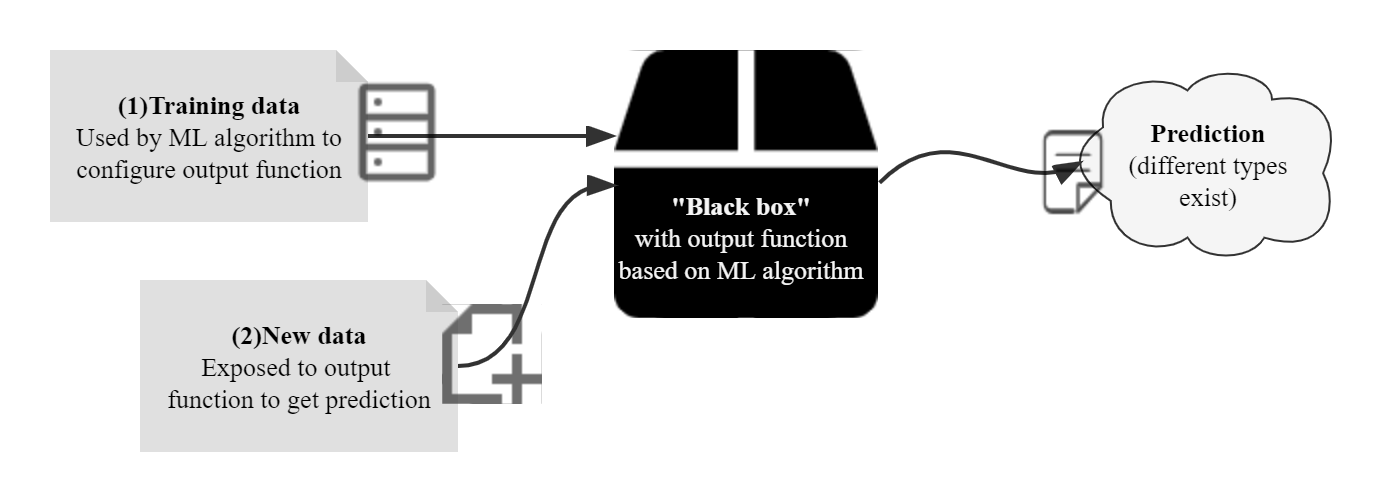
\includegraphics[width=5.5cm]{images/Black-box.png}
\caption{Black-box of AI}
\end{figure}
\column{.65\textwidth}
\begin{figure}
\centering
% Requires \usepackage{graphicx}
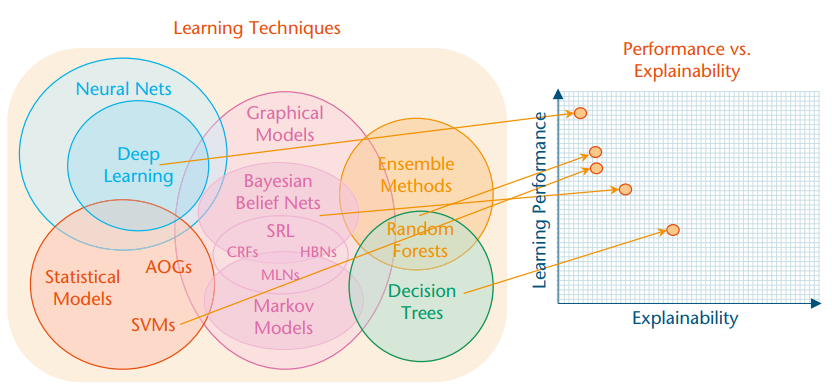
\includegraphics[width=6.3cm]{images/xai.png}
\caption{Learning Performance Versus Explainability Trade-Off of AI}
\end{figure}
\end{columns}
\end{frame}

\begin{frame}{Scheme}
\protect\hypertarget{scheme}{}
\begin{figure}

{\centering 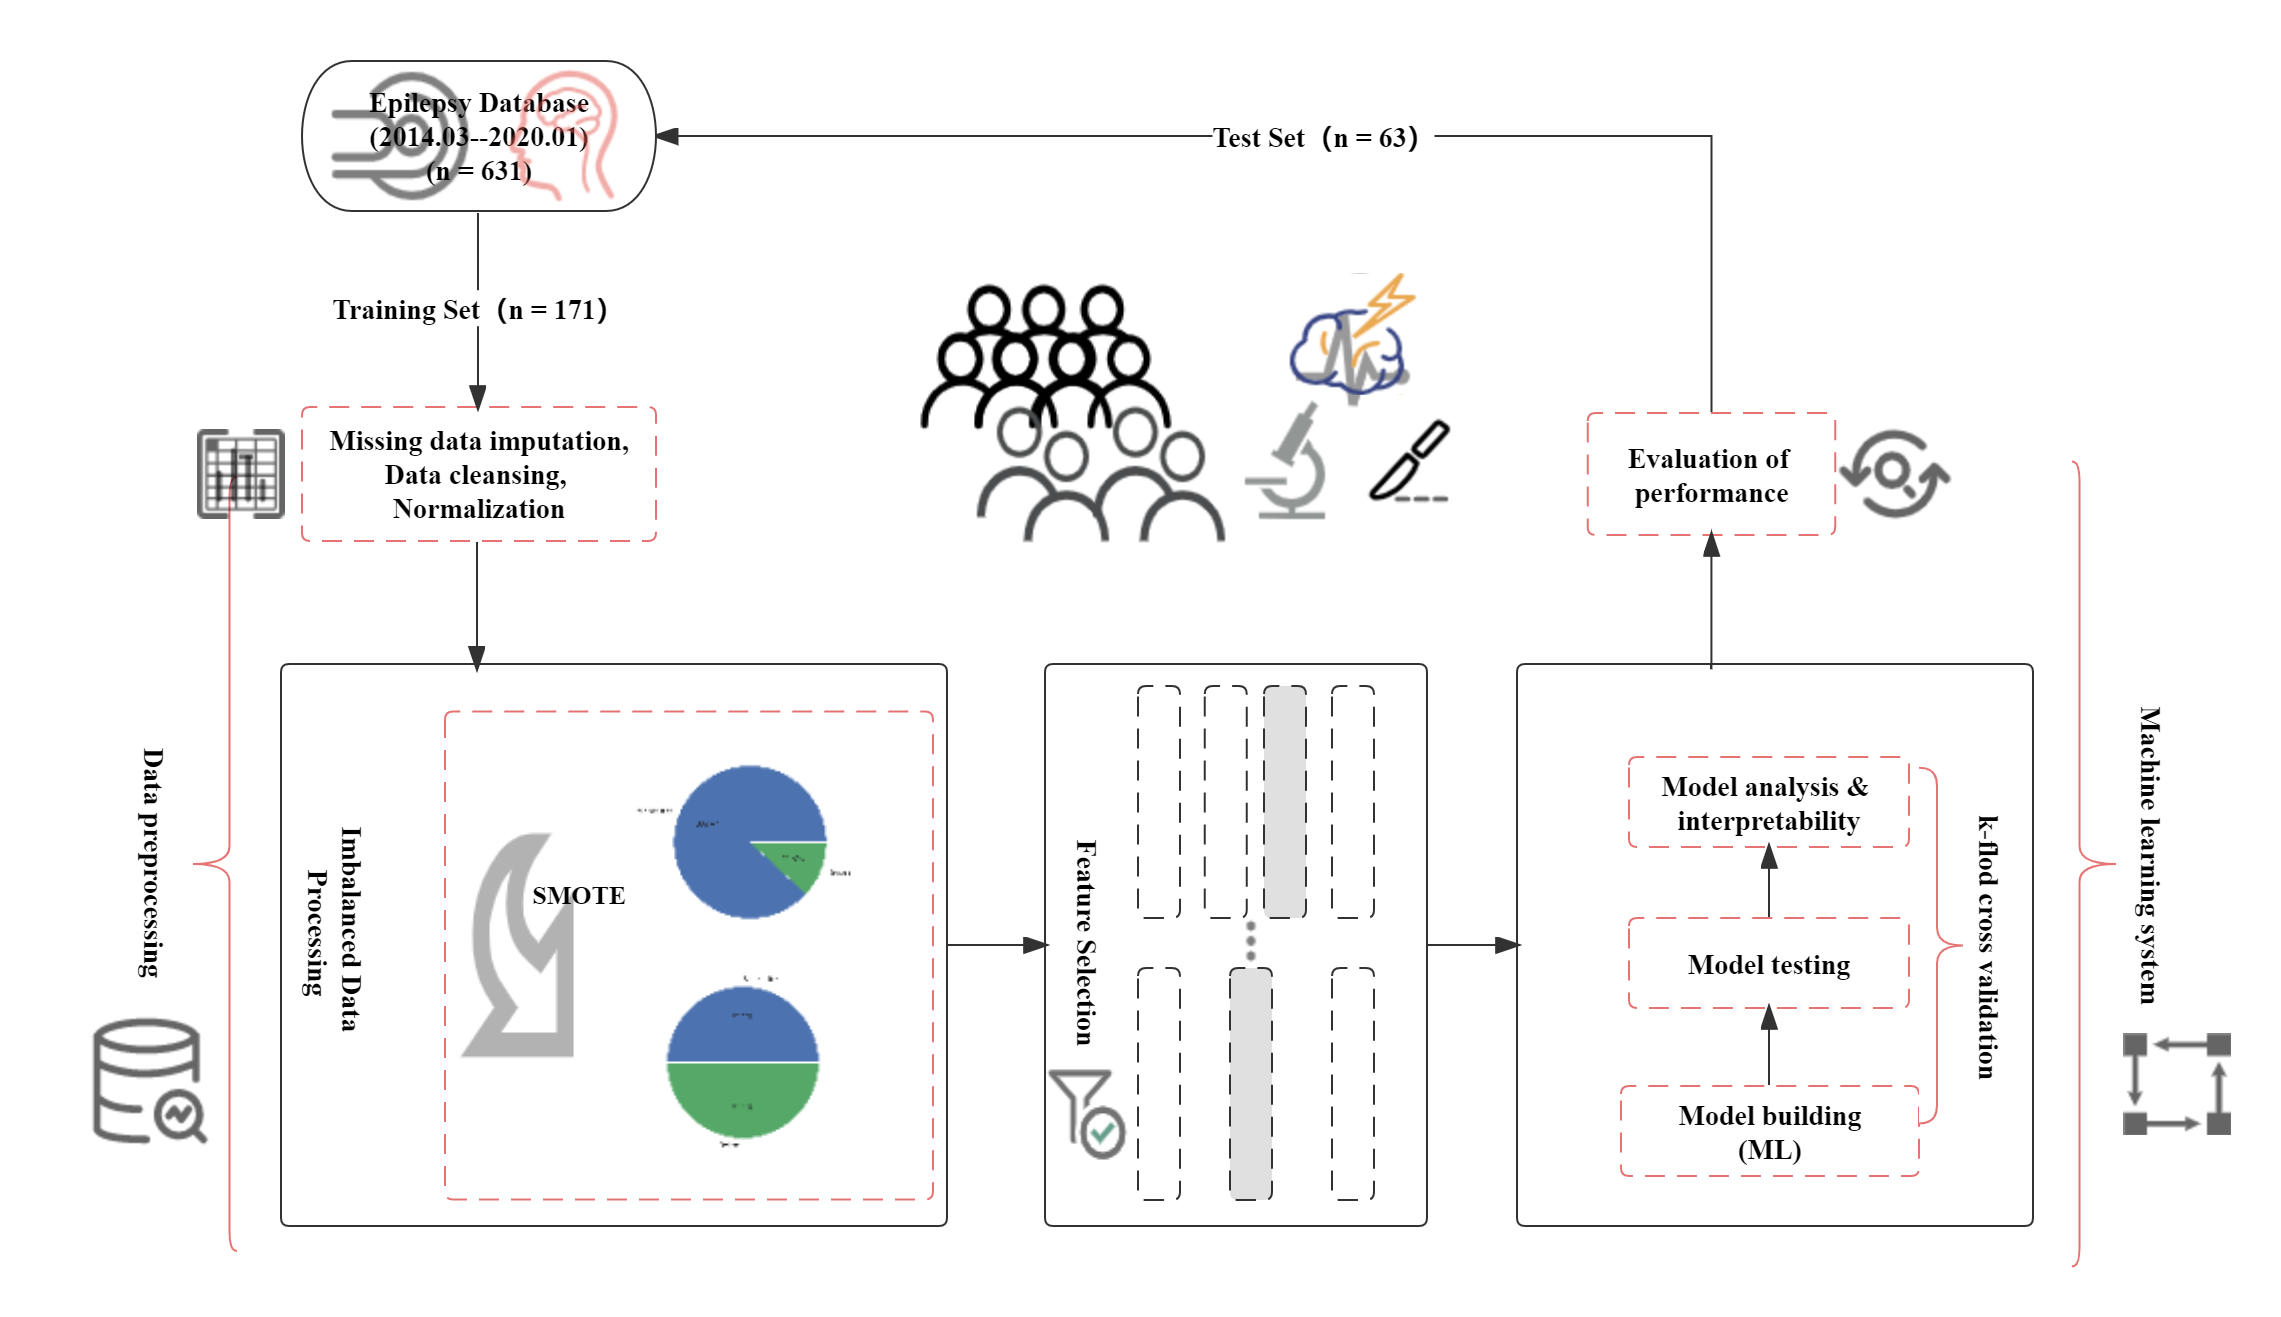
\includegraphics[width=0.85\linewidth]{images/TLE_EML_Flow} 

}

\caption{Flowchart of TLE Postsurgical IML}\label{fig:unnamed-chunk-3}
\end{figure}
\end{frame}

\hypertarget{the-data}{%
\section{The Data}\label{the-data}}

\begin{frame}{Combined of PET Radiomics and Clinical Features}
\protect\hypertarget{combined-of-pet-radiomics-and-clinical-features}{}
\begin{figure}

{\centering 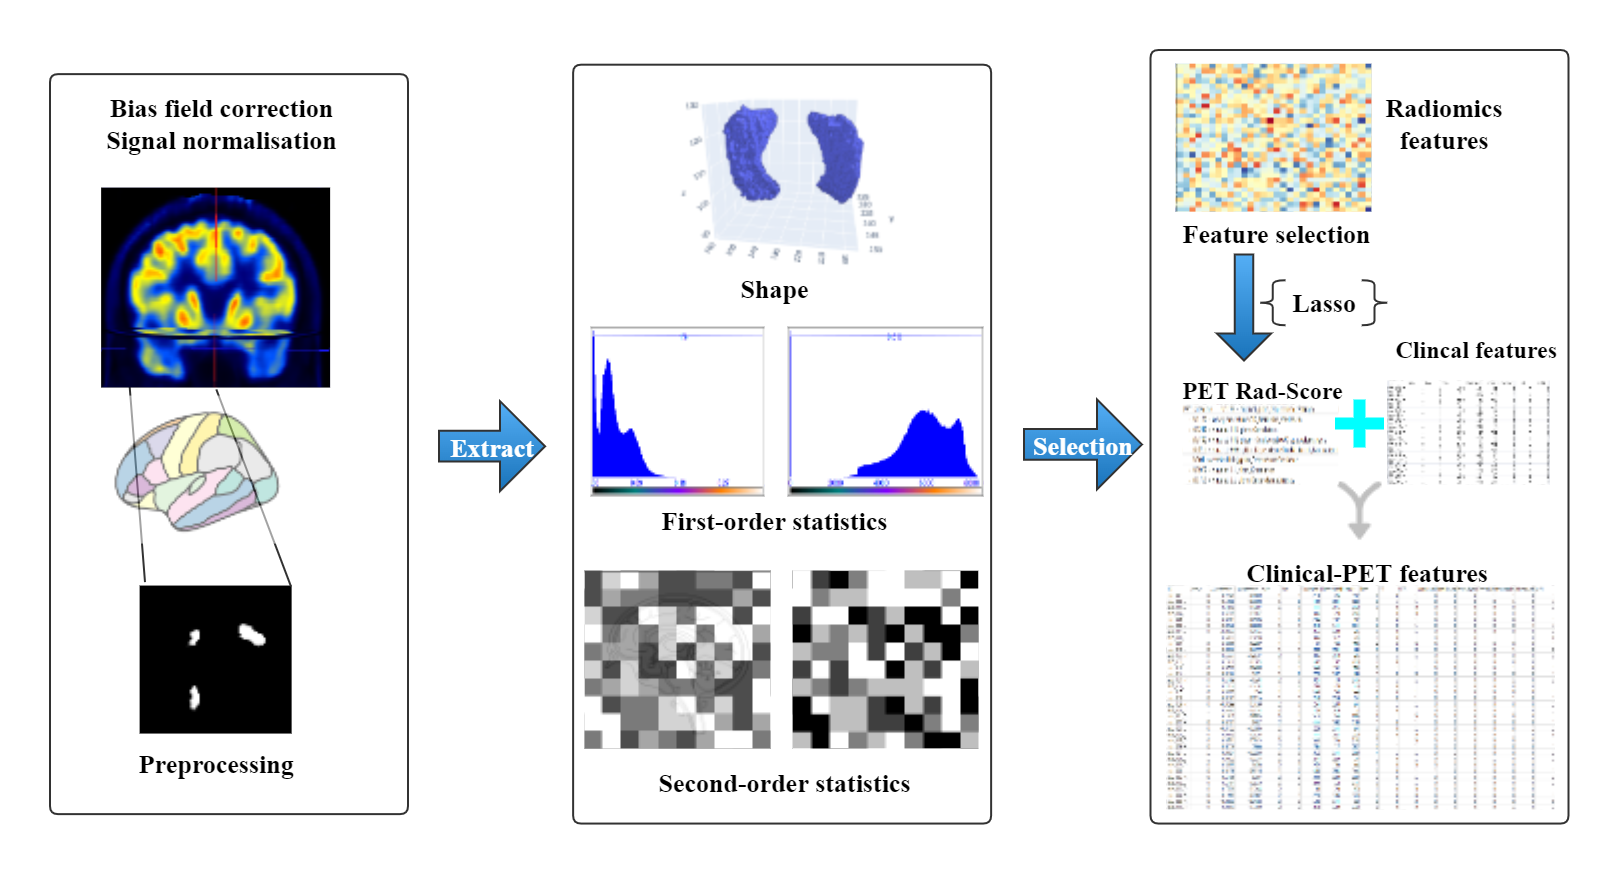
\includegraphics[width=1.1\linewidth]{images/PET_radiomics} 

}

\caption{PET Radiomics  Score and Clinical-PET Features}\label{fig:unnamed-chunk-4}
\end{figure}
\end{frame}

\begin{frame}{Exploratory Data Analysis}
\protect\hypertarget{exploratory-data-analysis}{}
\begin{figure}

{\centering 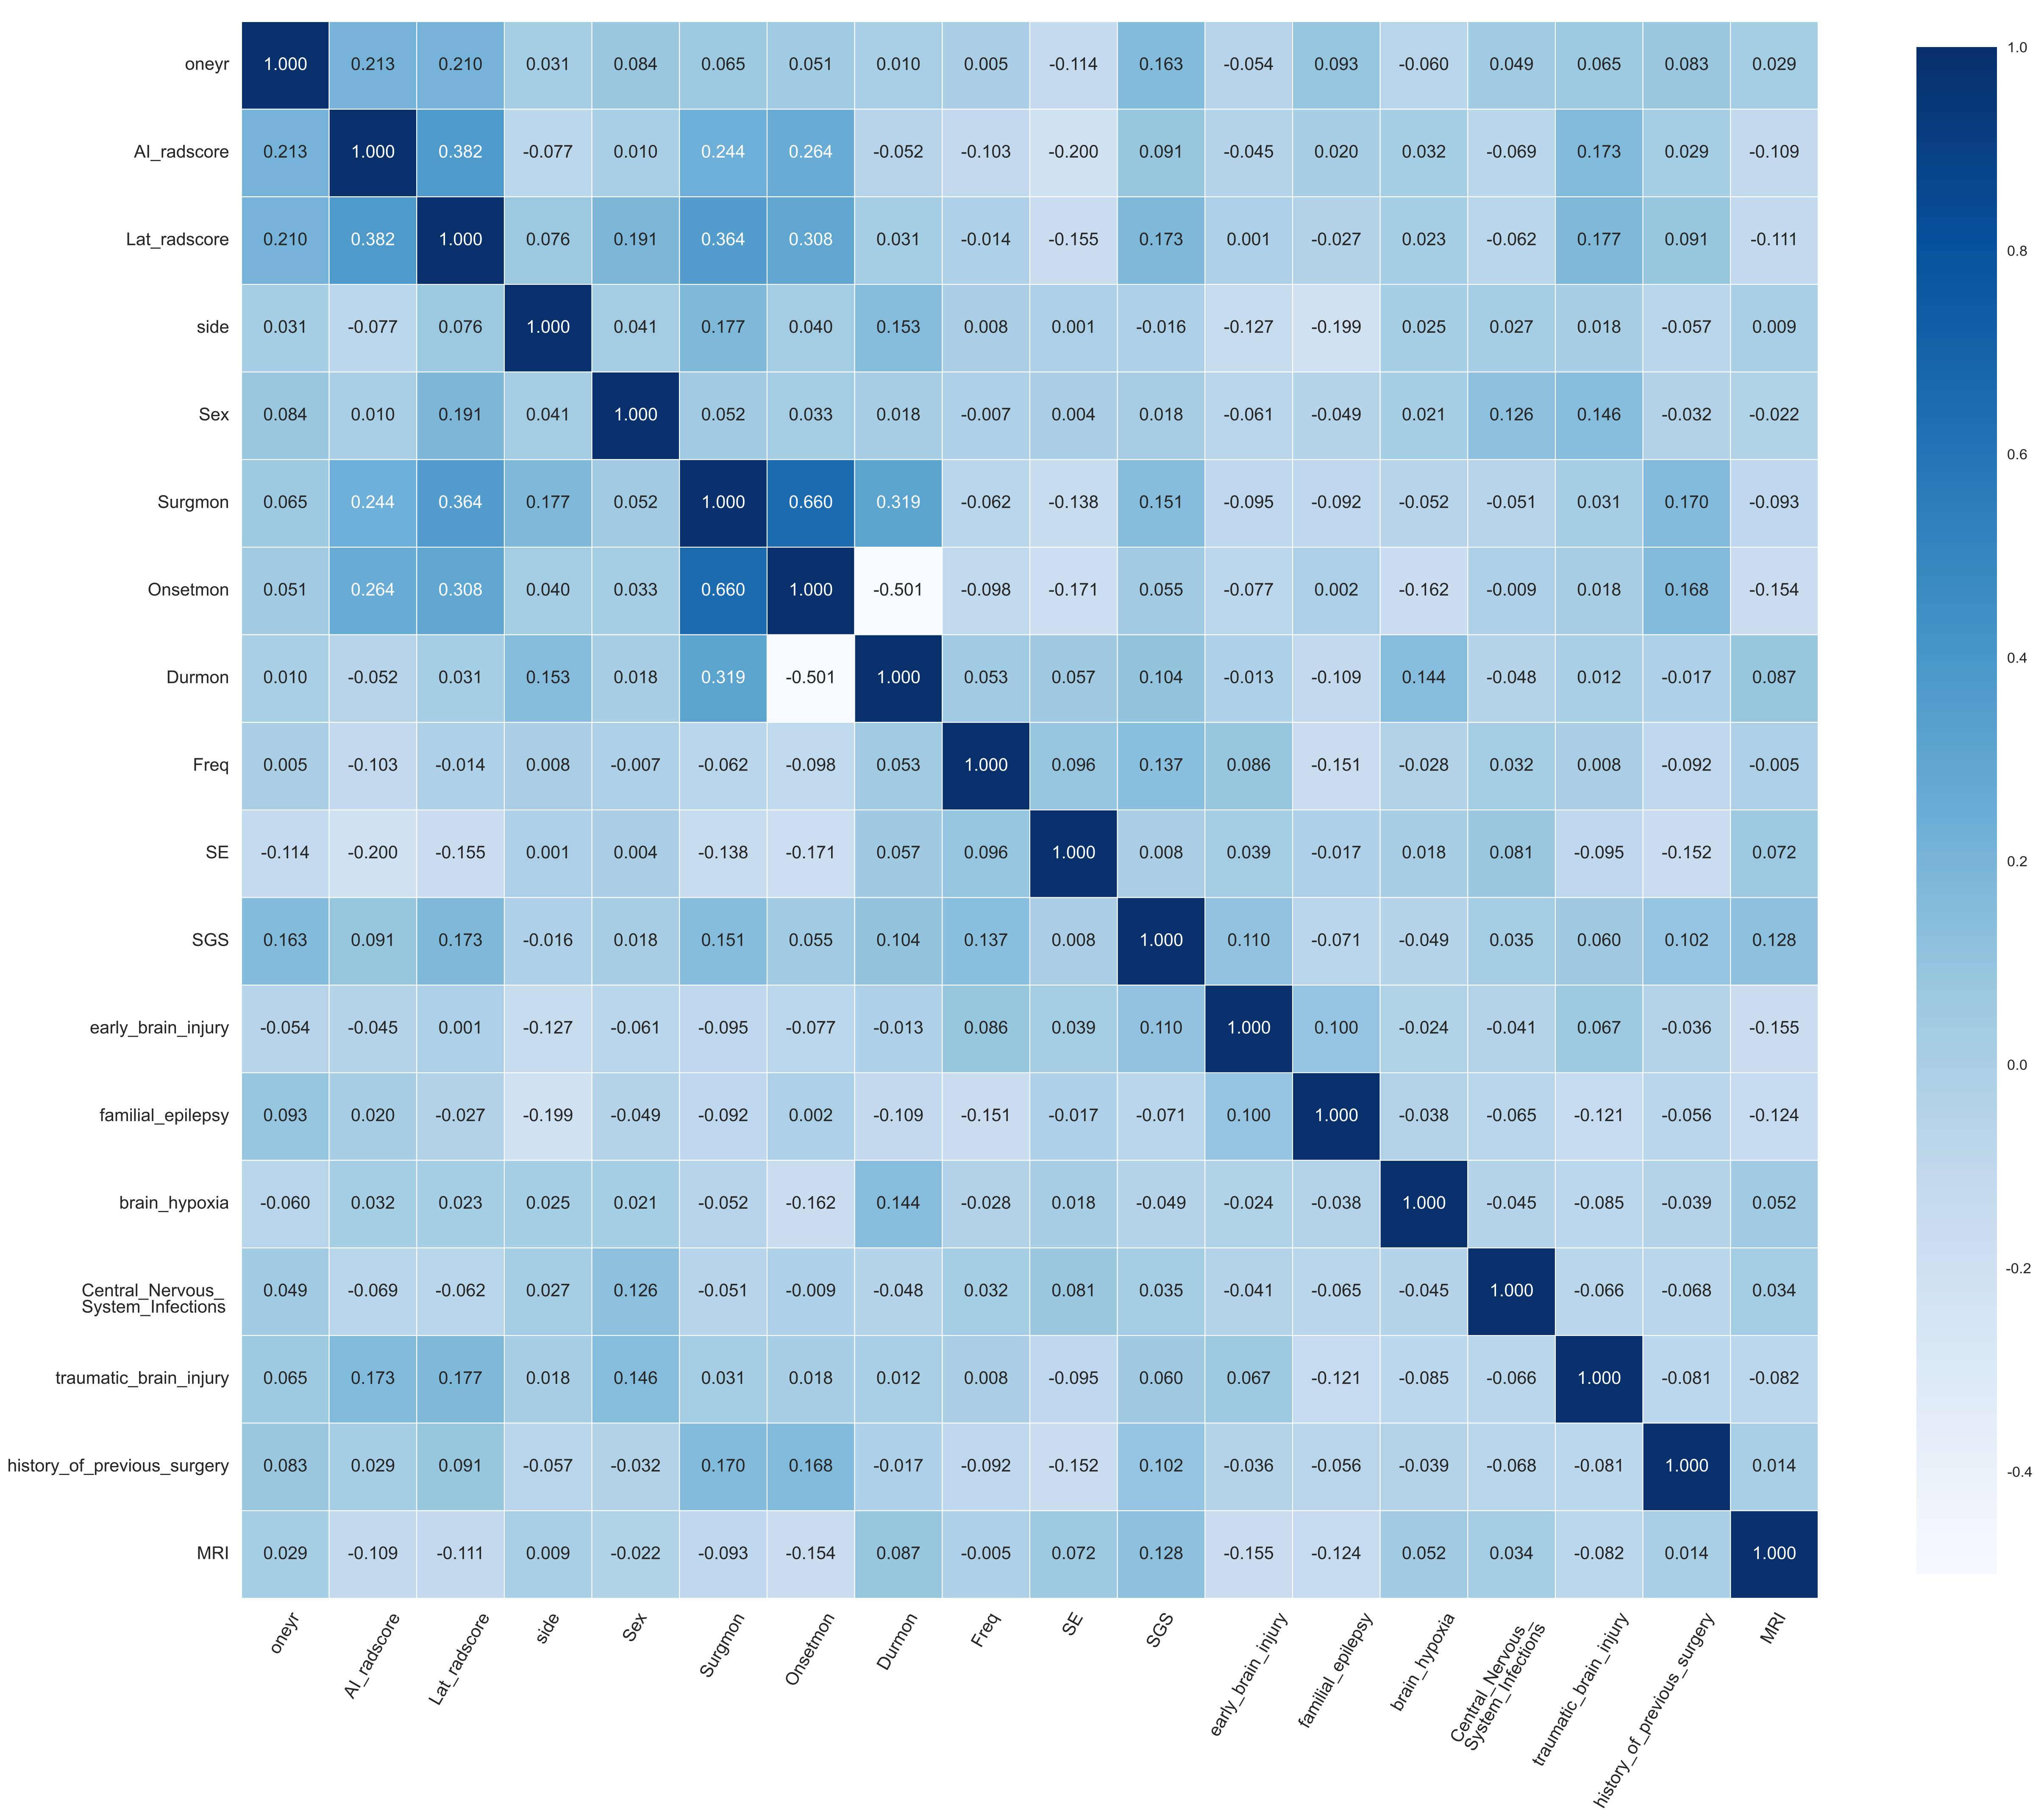
\includegraphics[width=0.6\linewidth]{images/heatplot} 

}

\caption{Heatmap of Clinical-PET Features}\label{fig:unnamed-chunk-5}
\end{figure}
\end{frame}

\hypertarget{the-model}{%
\section{The Model}\label{the-model}}

\begin{frame}{Benchmark}
\protect\hypertarget{benchmark}{}
\textbf{Table 1:} Performance Comparison Eleven ML Algorithms \centering
\tiny

\begin{table}[]
\begin{tabular}{lllllllll} \hline
Model                           & Accuracy & AUC   & Recall & Prec. & F1    & Kappa & MCC   & APC   \\ \hline
Ada Boost Classifier            & 0.883    & 0.789 & 0.4    & 0.433 & 0.393 & 0.345 & 0.357 & 0.59  \\ 
Extreme Gradient Boosting       & 0.884    & 0.777 & 0.3    & 0.4   & 0.333 & 0.287 & 0.295 & 0.607 \\
Random Forest Classifier        & 0.884    & 0.763 & 0.2    & 0.35  & 0.25  & 0.217 & 0.23  & 0.612 \\
Gradient Boosting Classifier    & 0.89     & 0.762 & 0.35   & 0.483 & 0.39  & 0.346 & 0.36  & 0.591 \\
Light Gradient Boosting Machine & 0.859    & 0.749 & 0.25   & 0.325 & 0.267 & 0.211 & 0.221 & 0.512 \\
Logistic Regression             & 0.878    & 0.669 & 0.05   & 0.1   & 0.067 & 0.055 & 0.059 & 0.448 \\
Extra Trees Classifier          & 0.884    & 0.662 & 0.1    & 0.2   & 0.133 & 0.118 & 0.127 & 0.443 \\
K Neighbors Classifier          & 0.865    & 0.646 & 0.2    & 0.2   & 0.183 & 0.14  & 0.149 & 0.283 \\
Linear Discriminant Analysis    & 0.884    & 0.642 & 0.1    & 0.2   & 0.133 & 0.119 & 0.128 & 0.418 \\
Naive Bayes                     & 0.251    & 0.586 & 0.9    & 0.129 & 0.226 & 0.014 & 0.072 & 0.332 \\
Decision Tree Classifier        & 0.798    & 0.584 & 0.3    & 0.264 & 0.259 & 0.158 & 0.167 & 0.218 \\
Std                             & 0.047    & 0.172 & 0.320  & 0.490 & 0.367 & 0.368 & 0.384 & 0.200 \\ \hline
\end{tabular}
\end{table}
\end{frame}

\begin{frame}[fragile]{AdaBoost Algorithm}
\protect\hypertarget{adaboost-algorithm}{}
\begin{figure}

{\centering 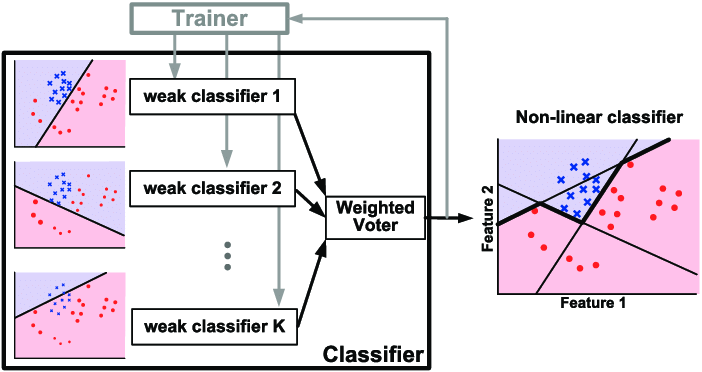
\includegraphics[width=0.8\linewidth]{images/AdaBoost} 

}

\caption{Illustration of AdaBoost Algorithm}\label{fig:unnamed-chunk-6}
\end{figure}

\begin{itemize}
\tightlist
\item
  \texttt{AdaBoostClassifier(algorithm=\textquotesingle{}SAMME\textquotesingle{},\ base\_estimator=None,\ learning\_rate=0.2,\ \ \ \ \ \ \ \ \ \ \ \ \ \ \ \ \ \ \ \ n\_estimators=230,\ random\_state=123)}
\end{itemize}
\end{frame}

\begin{frame}{Tuned AdaBoost}
\protect\hypertarget{tuned-adaboost}{}
\textbf{Table 2:} K-folds Cross-validation of the Selected AdaBoost
\centering \tiny

\begin{table}[]
\begin{tabular}{lllllllll}
\hline
\multicolumn{1}{c}{Tuned\_Ada} & \multicolumn{1}{c}{Accuracy} & \multicolumn{1}{c}{AUC} & \multicolumn{1}{c}{Recall} & \multicolumn{1}{c}{Prec.} & \multicolumn{1}{c}{F1} & \multicolumn{1}{c}{Kappa} & \multicolumn{1}{c}{MCC} & \multicolumn{1}{c}{APC} \\ \hline
1                              & 0.882                        & 0.733                   & 0.000                      & 0.000                     & 0.000                  & 0.000                     & 0.000                   & 0.361                   \\ 
2                              & 1.000                        & 1.000                   & 1.000                      & 1.000                     & 1.000                  & 1.000                     & 1.000                   & 1.000                   \\
3                              & 0.824                        & 0.550                   & 0.000                      & 0.000                     & 0.000                  & -0.085                    & -0.091                  & 0.183                   \\
4                              & 0.875                        & 0.893                   & 0.000                      & 0.000                     & 0.000                  & 0.000                     & 0.000                   & 0.500                   \\
5                              & 0.938                        & 0.929                   & 0.500                      & 1.000                     & 0.667                  & 0.636                     & 0.683                   & 0.750                   \\
6                              & 0.938                        & 0.964                   & 0.500                      & 1.000                     & 0.667                  & 0.636                     & 0.683                   & 0.833                   \\
7                              & 0.875                        & 0.554                   & 0.000                      & 0.000                     & 0.000                  & 0.000                     & 0.000                   & 0.321                   \\
8                              & 0.938                        & 0.964                   & 0.500                      & 1.000                     & 0.667                  & 0.636                     & 0.683                   & 0.833                   \\
9                              & 0.938                        & 1.000                   & 0.500                      & 1.000                     & 0.667                  & 0.636                     & 0.683                   & 1.000                   \\
10                             & 0.938                        & 0.679                   & 0.500                      & 1.000                     & 0.667                  & 0.636                     & 0.683                   & 0.591                   \\
Mean                           & 0.914                        & 0.827                   & 0.350                      & 0.600                     & 0.433                  & 0.410                     & 0.432                   & 0.637                   \\
Std                            & 0.047                        & 0.172                   & 0.320                      & 0.490                     & 0.367                  & 0.368                     & 0.384                   & 0.200       \\ \hline           
\end{tabular}
\end{table}
\end{frame}

\hypertarget{the-explanation}{%
\section{The Explanation}\label{the-explanation}}

\begin{frame}{Permutation Importance}
\protect\hypertarget{permutation-importance}{}
\begin{figure}

{\centering 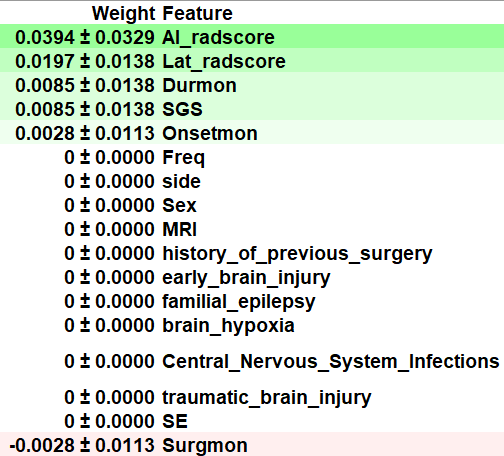
\includegraphics[width=0.6\linewidth]{images/eli5} 

}

\caption{Permutation Importance of AdaBoost}\label{fig:unnamed-chunk-7}
\end{figure}
\end{frame}

\begin{frame}{Partial Dependence Plot}
\protect\hypertarget{partial-dependence-plot}{}
PDP plots:

\begin{itemize}[<+->]
\item \begin{columns}
\column{.4\textwidth}
\begin{figure}
\centering
% Requires \usepackage{graphicx}
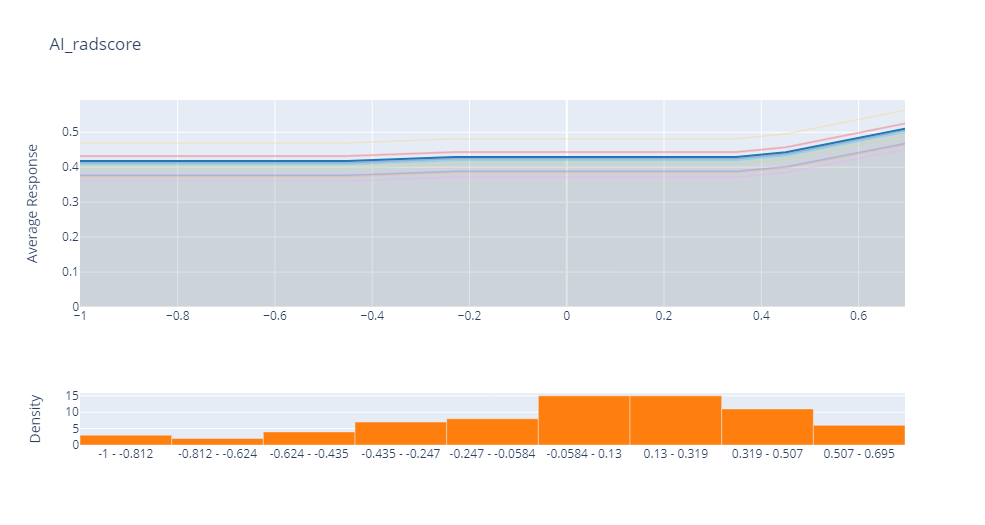
\includegraphics[width=6cm]{images/pdp_1.png}
\end{figure}
\column{.5\textwidth}
\begin{figure}
\centering
% Requires \usepackage{graphicx}
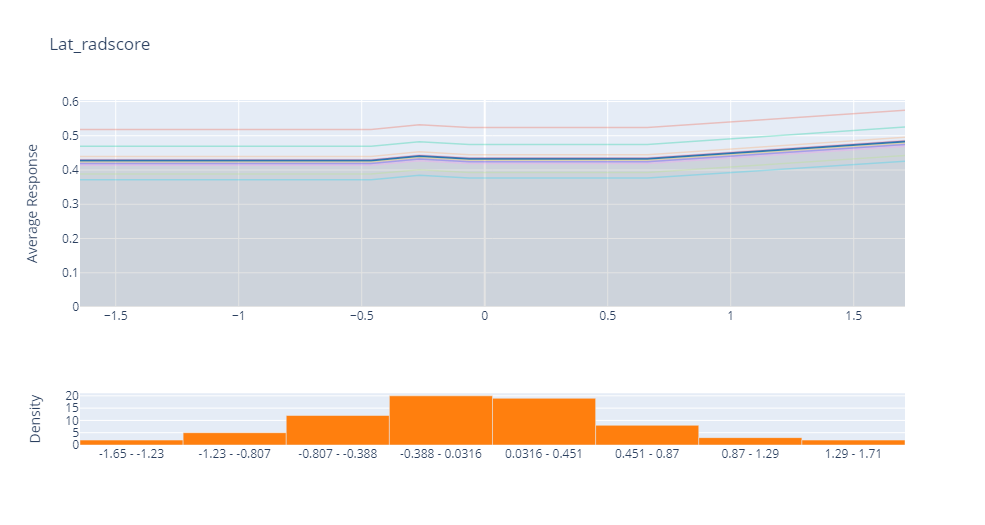
\includegraphics[width=6cm]{images/pdp_2.png}
\end{figure}
\end{columns}
\end{itemize}
\end{frame}

\hypertarget{conclusion}{%
\section{Conclusion}\label{conclusion}}

\begin{frame}{Key Points}
\protect\hypertarget{key-points}{}
\begin{itemize}[<+->]
\item Metabolic radiomics are helpful to predict the postsurgical seizure outcomes;
\bigskip
\item Combination of PET Radiomics and Clinical Features are more robust;
\bigskip
\item IML technique can further deepen the understanding of the principle of ML models and the decision-making process for professional and intuitive interpretation
\end{itemize}
\end{frame}

\begin{frame}{Limitations}
\protect\hypertarget{limitations}{}
\begin{itemize}[<+->]
\item More data, especially external validation cohort;
\bigskip
\item Fusion of PET/MRI multimodal imaging;
\bigskip
\item Other subtypes of drug-resistant epilepsy
\end{itemize}
\end{frame}

\begin{frame}{}
\protect\hypertarget{section}{}
For more theoretical approaches to machine learning model explanation,
see
\href{https://christophm.github.io/interpretable-ml-book/}{Interpretable
Machine Learning: A Guide for Making Black Box Models Explainable},refer
to\citep{beghi2019global},\citep{rajpurkar2021deep},\citep{mlr3book},\citep{molnar2022}.

\bigskip

\textbf{Email:}
\href{mailto:wane199@outlook.com}{\nolinkurl{wane199@outlook.com}}
\end{frame}

\begin{frame}{}
\protect\hypertarget{section-1}{}
\begin{center}
  \emph{\textbf{\Huge{{THANKS !}}}}
\end{center}
%
\begin{tikzpicture}[remember picture,overlay]
\node[inner sep = 0pt, outer sep = 0pt,opacity=0.65]
  at (current page.center)
  {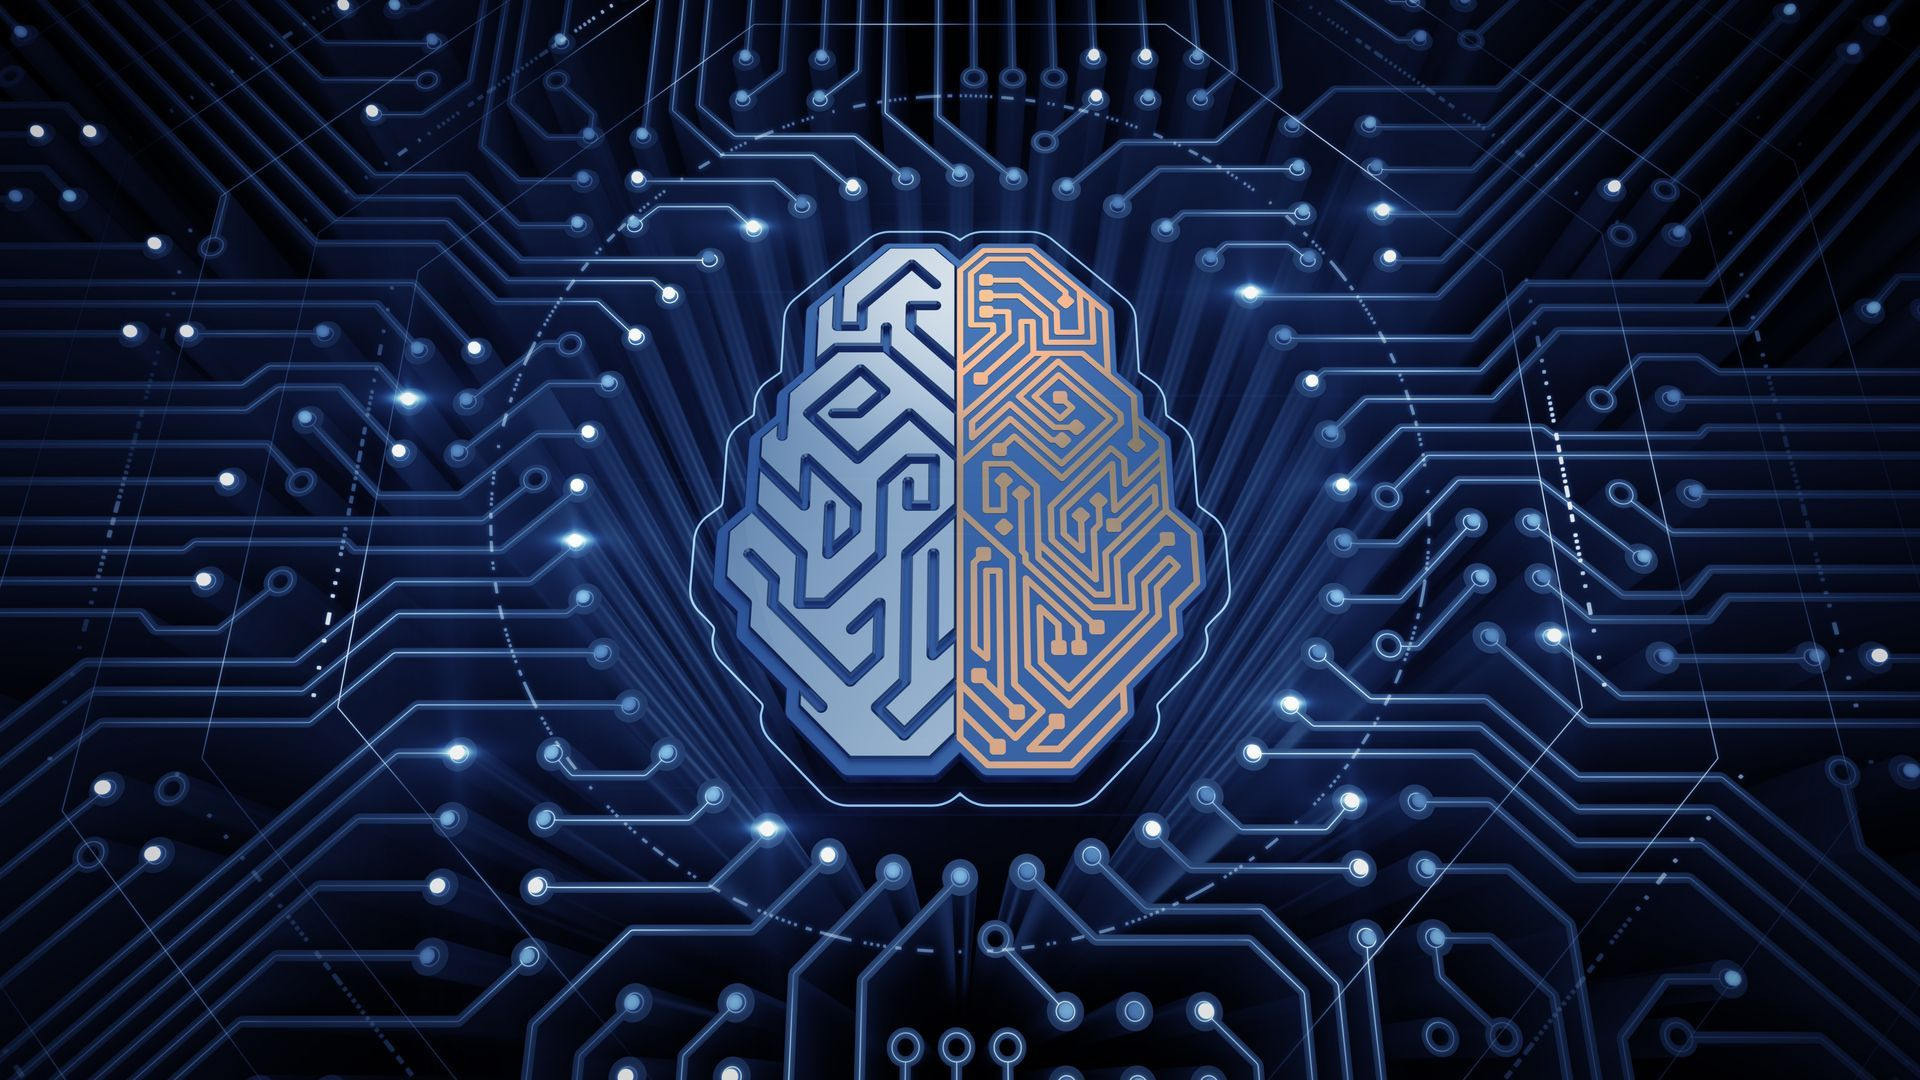
\includegraphics[width=\paperwidth,height=\paperheight]{images/AI.jpg}};
\end{tikzpicture}%
\end{frame}

\renewcommand\refname{References}
\begin{frame}[allowframebreaks]{References}
  \bibliographytrue
  \bibliography{refer.bib}
\end{frame}

\end{document}
